\section{Testing}
We tested three Mini-MAC implementations on the Texas Instruments MSP430F5529 microcontroller. The speed and power of this device makes it an appropriate test platform for CAN security software.

\subsection{Purpose}

The purpose of our tests is to evaluate the suitability of HMAC-based message authentication for nodes on the CAN bus. Small memory, RAM and performance overhead is ideal, on the basis that ECUs are low-resource devices. The three hash functions selected are compared for two reasons 1) Performance and security are functions of the hash function selected as a base 2) Overlaying Mini-MAC onto HMAC should incur a minimal performance penalty regardless of the hash selected.

\subsection{Methods}

The tests performed were executing the Mini-MAC construction protocol over a variety of inputs, repeated 1000 times. This test, although simple, is sufficient to characterize the performance of the protocol. The metrics recorded are code size, memory usage, execution speed, and bus utilization.

Statistics on message traffic were collected from a 2010 Toyota Prius with a CAN-bus sniffer program  based on an Arudiuno Uno platform and connected via an OBD-II CAN transceiver shield.

A counter register on the MSP430 generates execution time values. A 32kHz clock increments this counter, which provides approximate millisecond execution time values. There may be a +/-0.03ms inaccuracy in this value depending on the time it takes to read the counter.

RAM and memory usage figures are generated at compile-time. Texas Instruments Code Composer v6 provides values for both after code is generated.

\subsection{Results}

Table 1 shows that even for a group key protocol, traditional HMAC adds at least two extra CAN messages for every data message sent. Lin-MAC MD5 sends an additional two messages per every user. Mini-MAC sends no additional messages. B represents a value in bytes, b is a value in bits, while ms represents a value in milliseconds.
	
	\begin{table}
	\centering
	\caption{MAC Bus Traffic Addition}
	\vspace{8pt}
	\begin{tabular}{|l|c|}\hline%
	\bfseries Function & \bfseries Add. Traffic (b) \\\hline \csvreader[late after line=\\]%
		{tables/bus_addition.csv}{function=\function,at=\at}%
		{\function & \at}%
		\hline
	\end{tabular}
	\end{table}

	\begin{table*}	
	\centering	
	\caption{Mini-MAC Overhead Relative to HMAC}
	\vspace{8pt}
	\begin{tabular}{|l|c|c|c|}\hline%
	\bfseries Hash & \bfseries Code Size (B) & \bfseries RAM Use (B) & \bfseries Execution Time (ms)\\\hline \csvreader[late after line=\\]%
		{tables/overhead.csv}{hash=\hash,code_size=\code_size,ram_size=\ram_size,exec_time=\exec_time}% 
		{\hash & \code_size & \ram_size & \exec_time}%
		\hline
	\end{tabular}
	\end{table*}
	
	\begin{table}
	\centering
	\caption{Approximate Execution Time of Mini-MAC Construction}
	\vspace{8pt}
	\begin{tabular}{| @{}l | S[table-format=2.1] | @{}}
		%\toprule
		\hline 
		\hspace{2pt}\textbf{Hash} & {\textbf{Exec. Time (ms)}} \\
		\hline 
		\hspace{2pt}MD5 & 7.5 \\
		\hspace{2pt}SHA1 & 28.0 \\
		\hspace{2pt}SHA2 & 69.6 \\ 
		%\bottomrule
		\hline
	\end{tabular}	
	\end{table}
	
	\begin{figure}
		\centering
		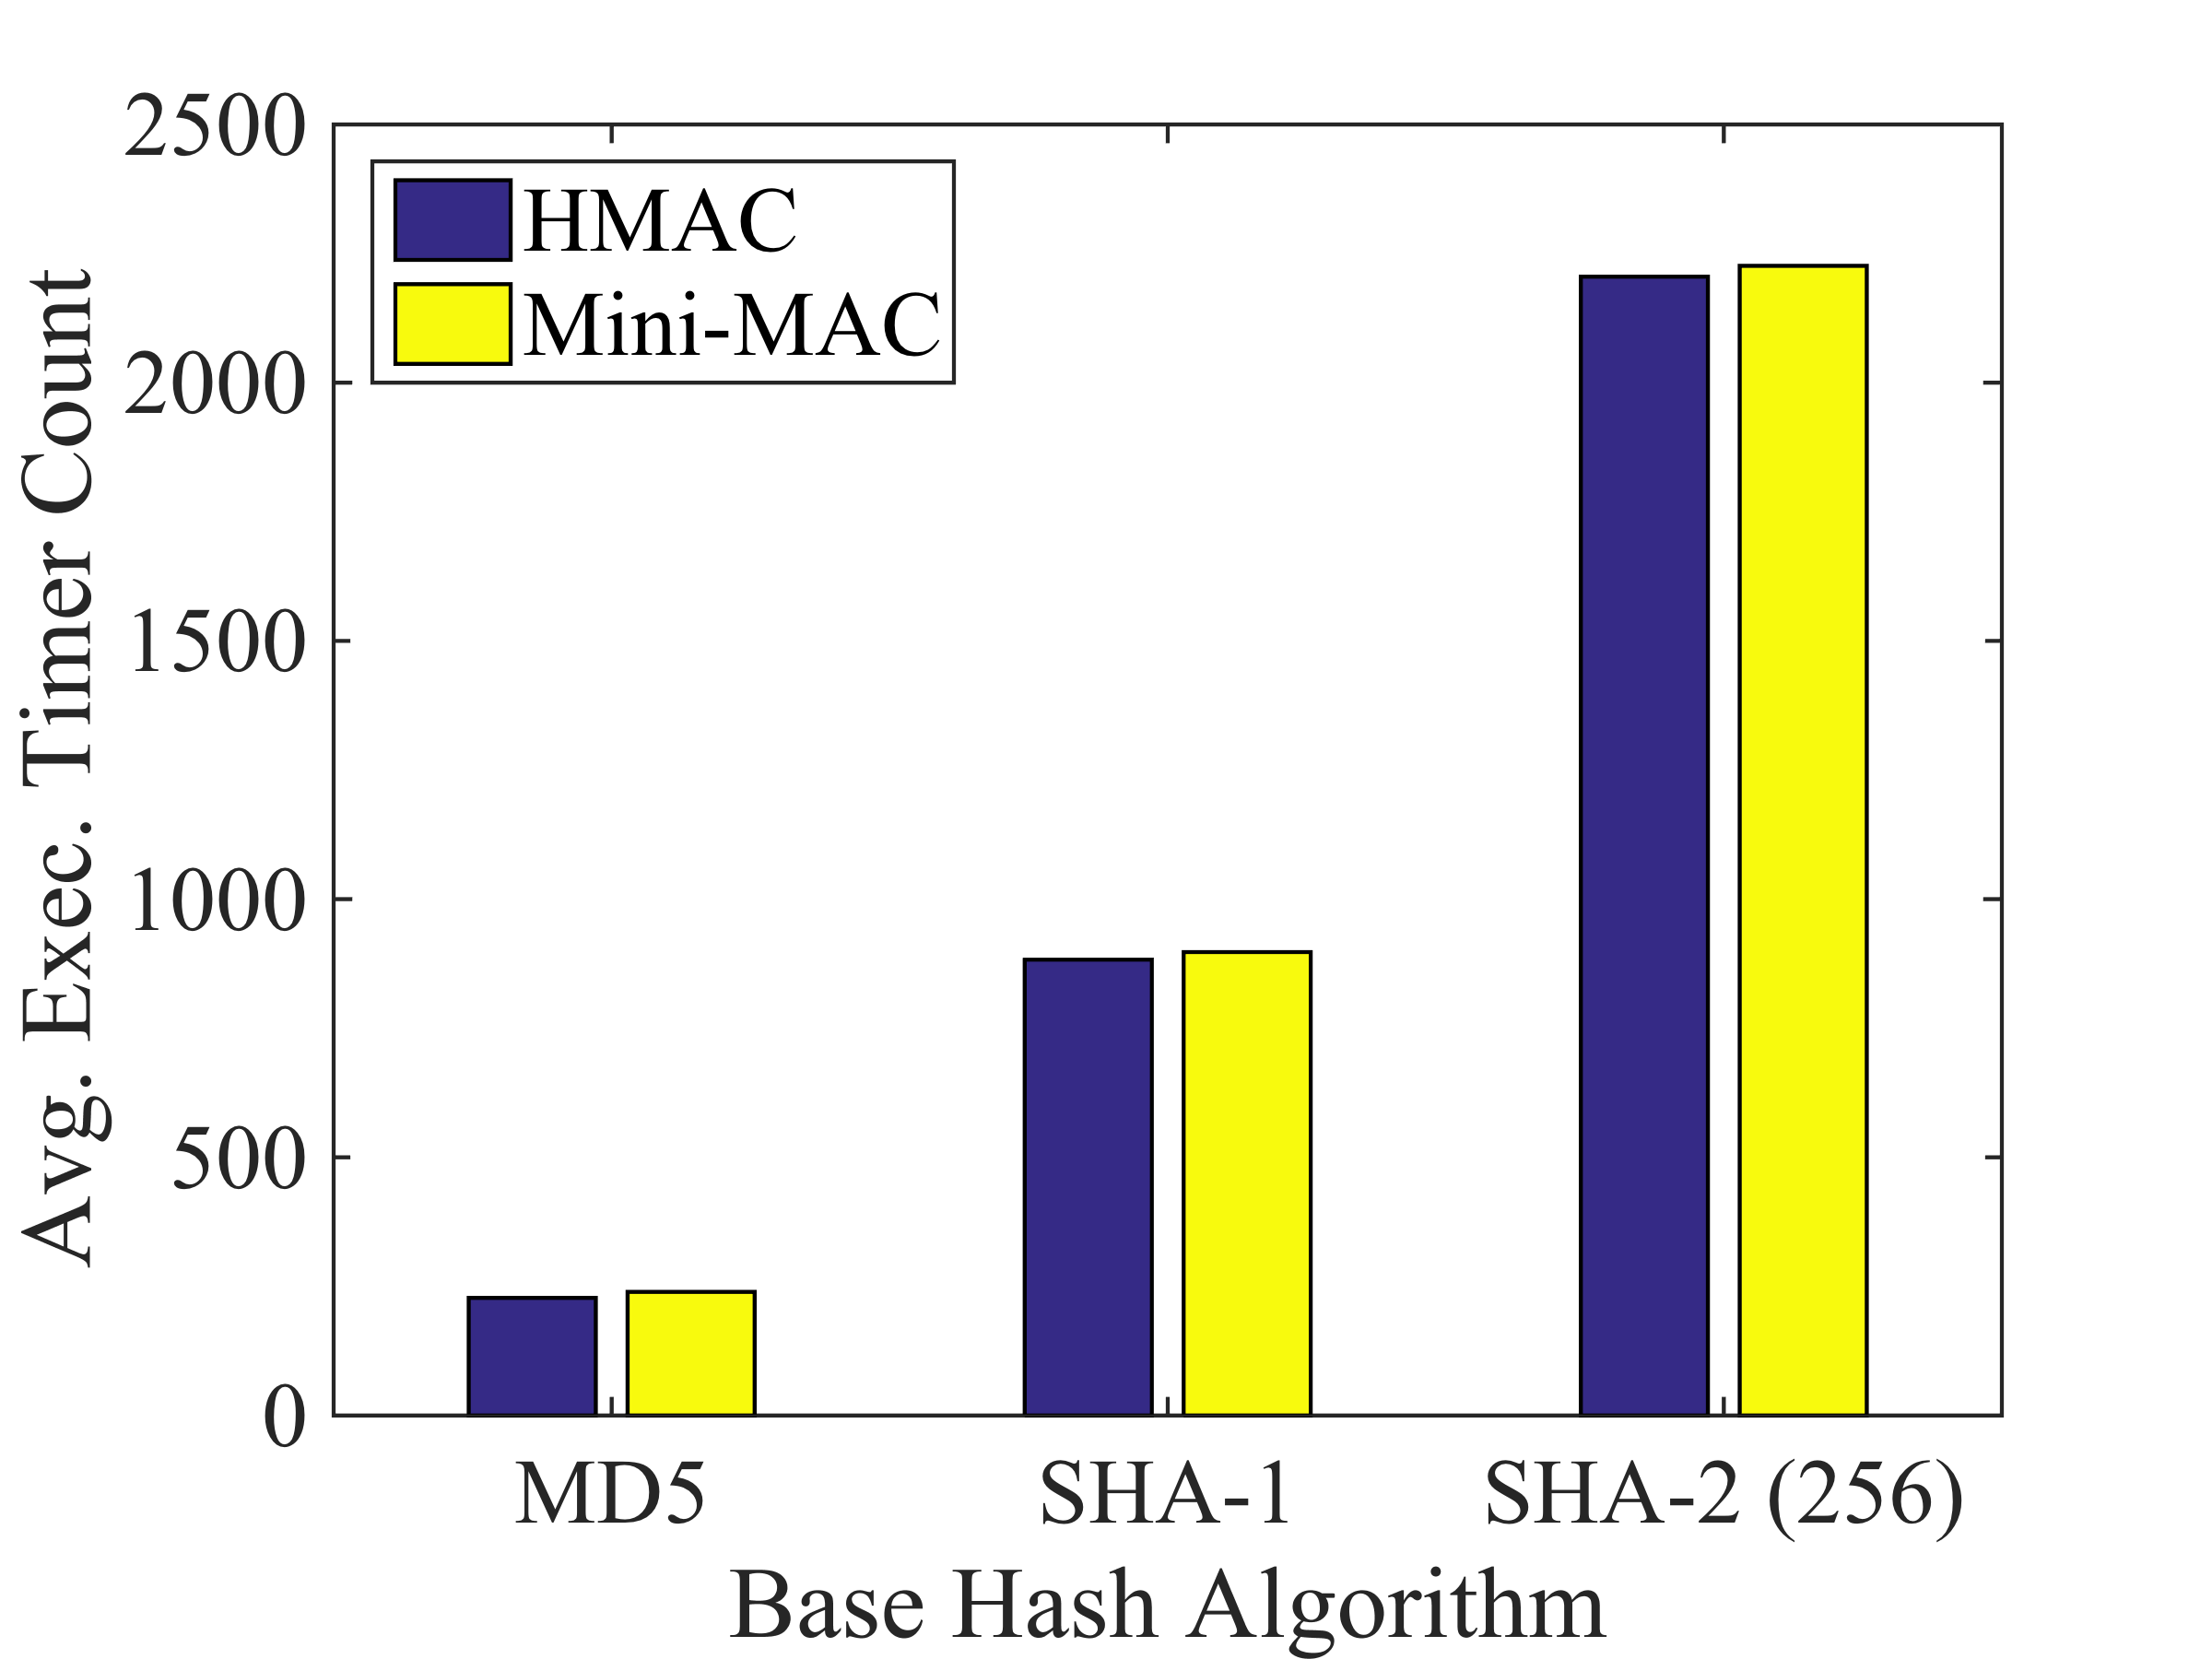
\includegraphics[width=\columnwidth]{figures/exec_cycles.png}
		\caption{Execution Time Comparison of Mini-MAC Construction}
	\end{figure}
	
	\begin{figure}
		\centering
		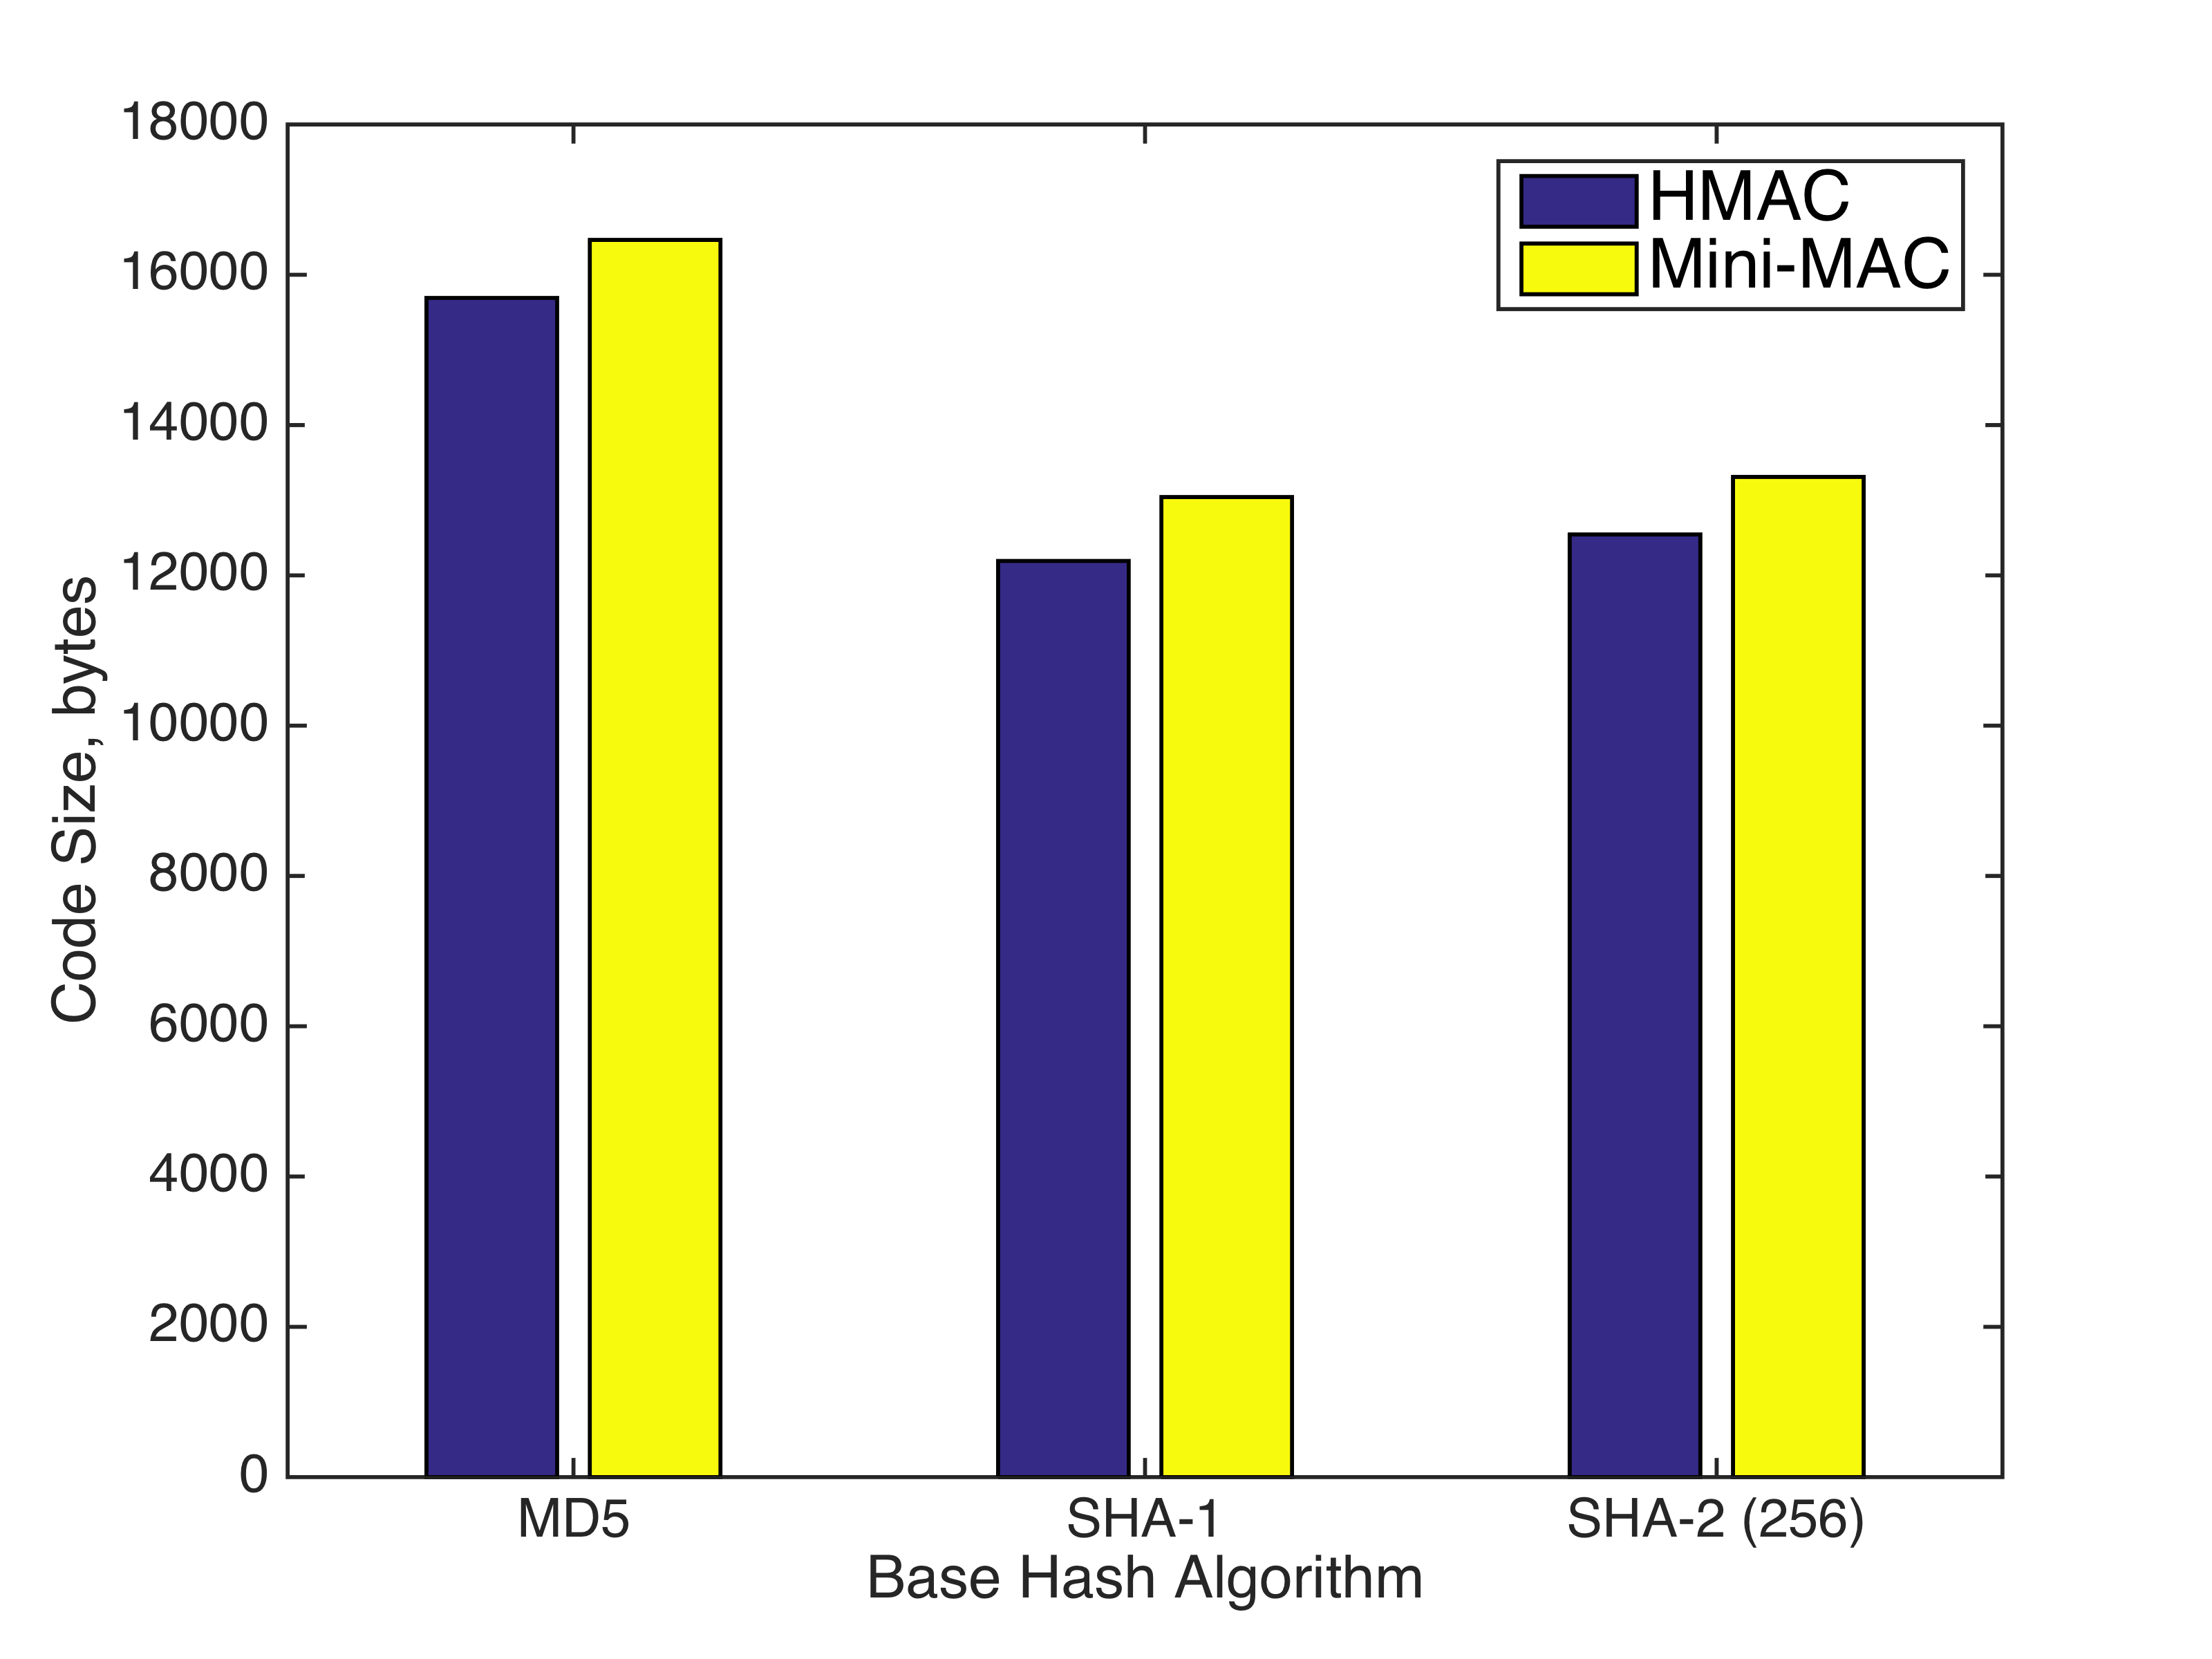
\includegraphics[width=\columnwidth]{figures/code_size.png}
		\caption{Code Size Comparison of Mini-MAC Code}
	\end{figure}
	
	\begin{figure}
		\centering
		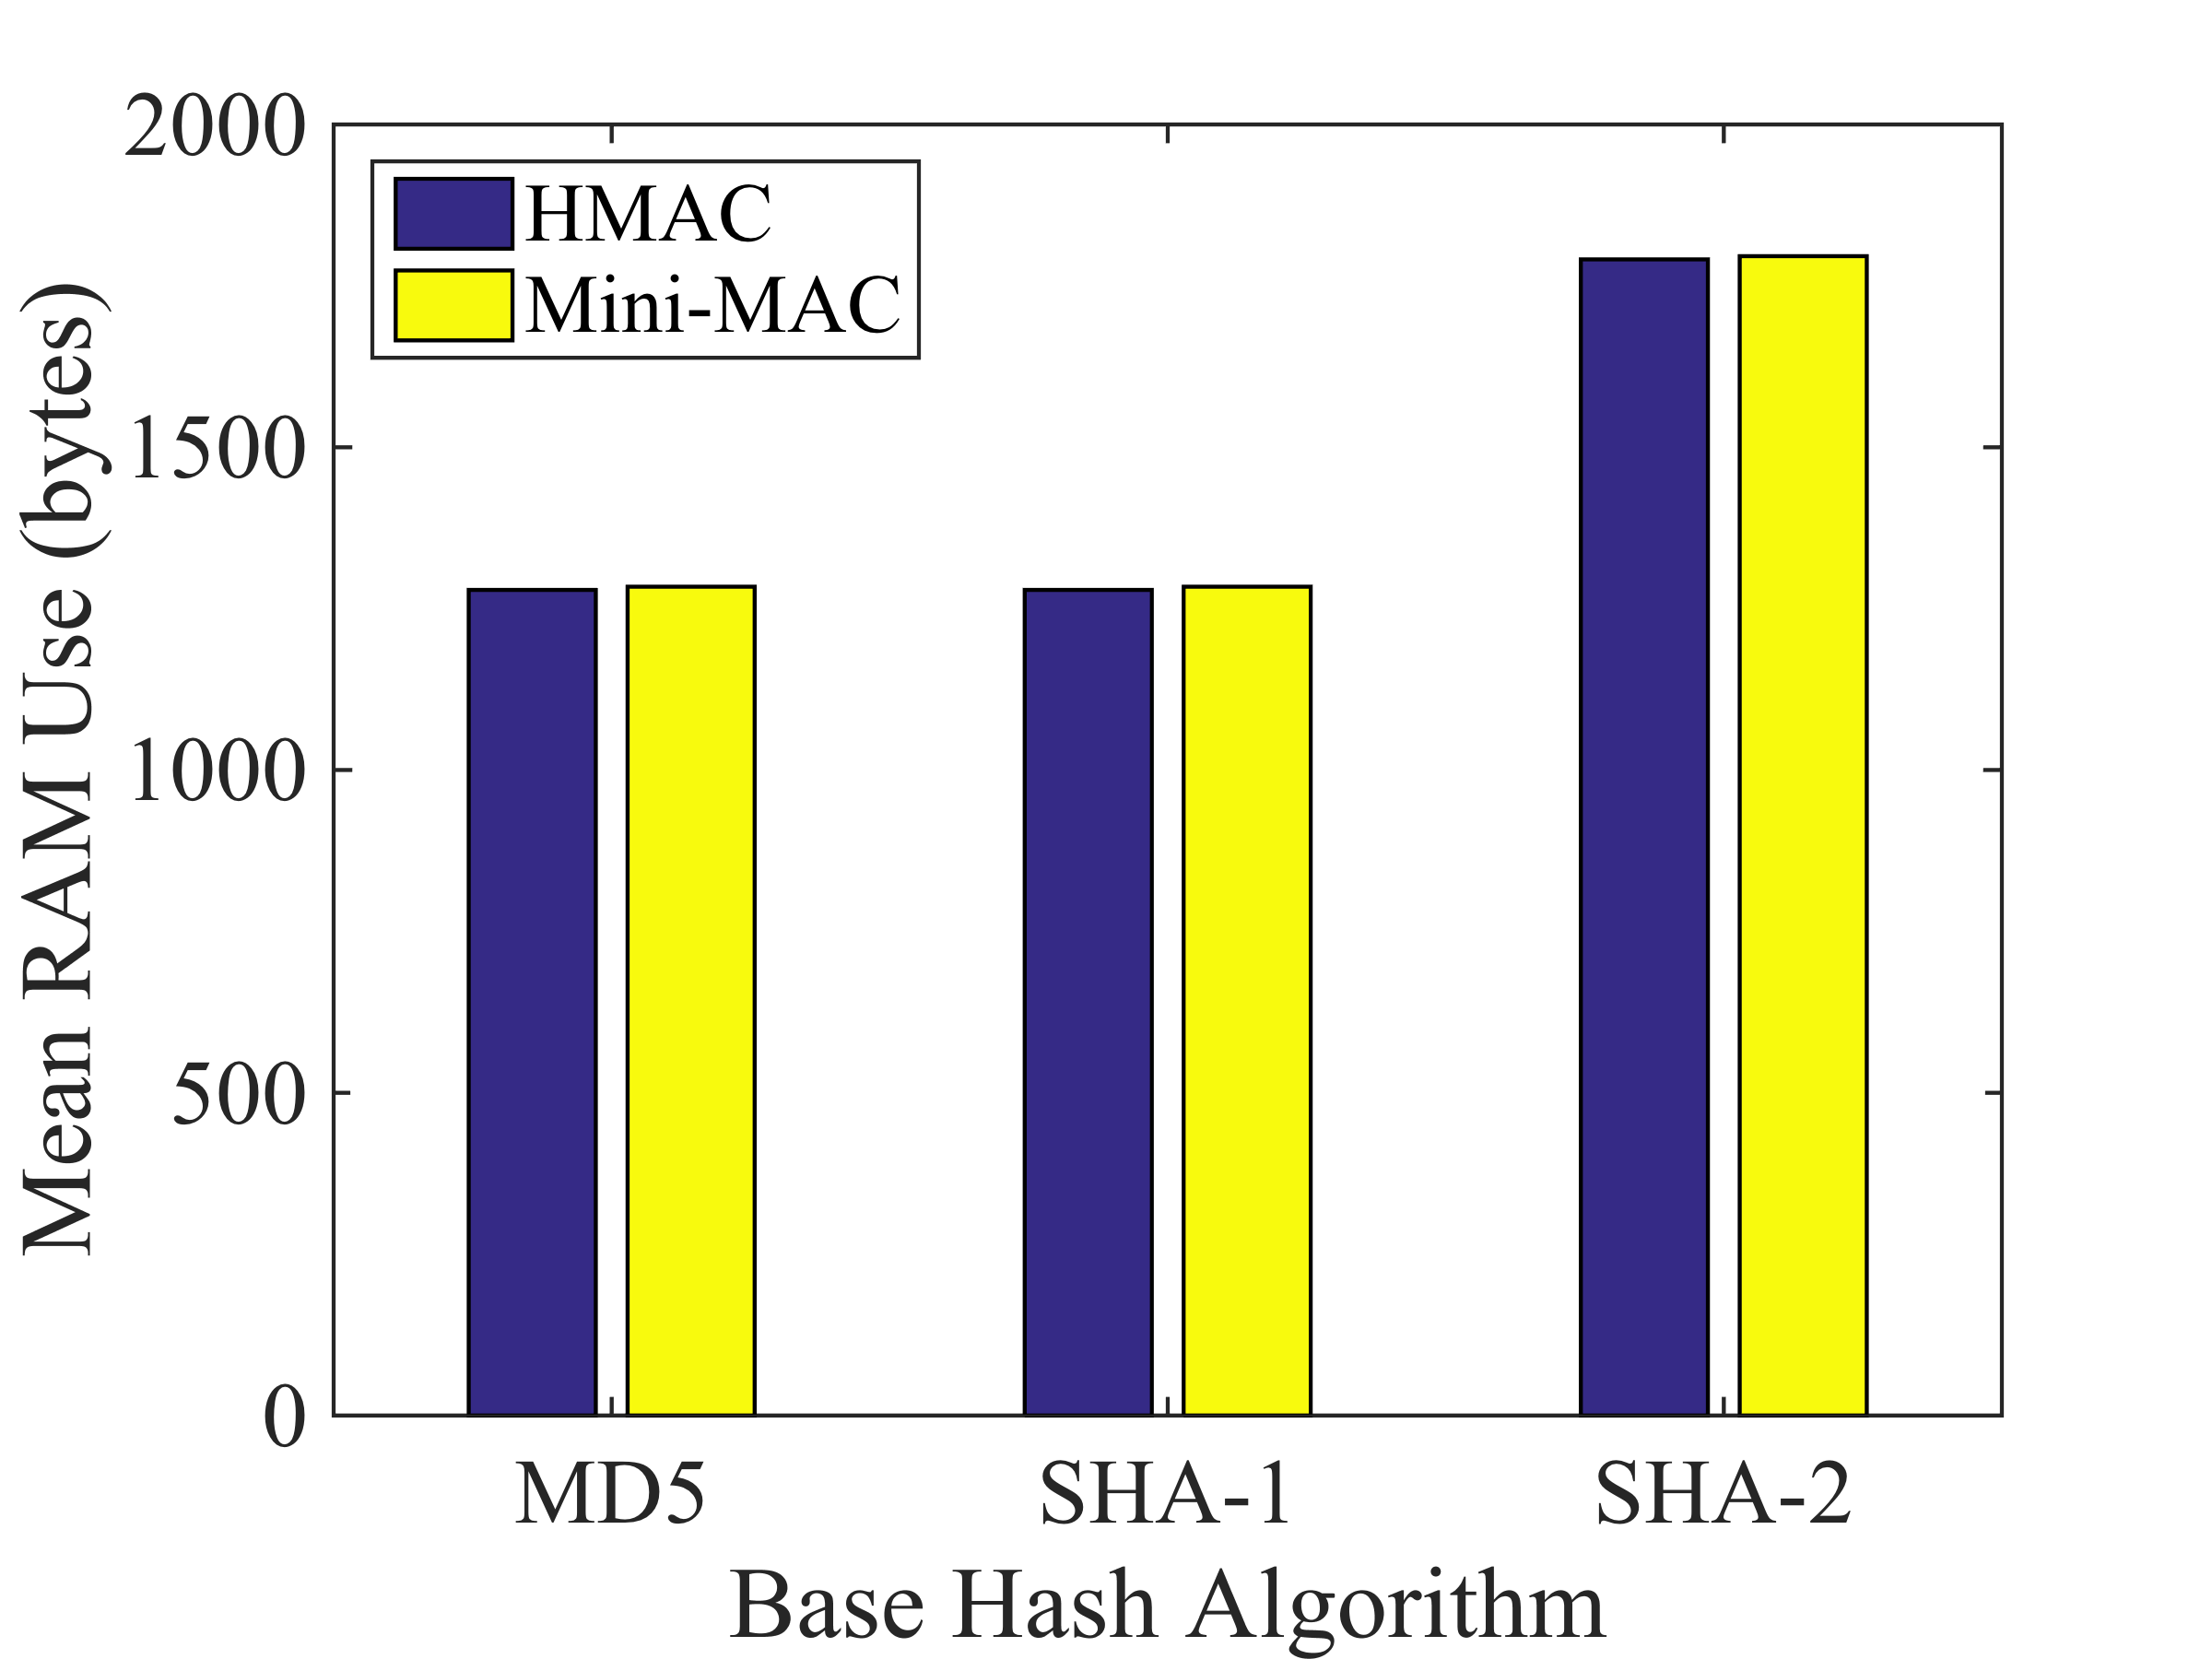
\includegraphics[width=\columnwidth]{figures/ram_usage.png}
		\caption{RAM Usage Comparison of Mini-MAC Code}
	\end{figure}
	